\documentclass{article}


\usepackage[T1]{fontenc}
\usepackage[utf8]{inputenc}
\usepackage[english]{babel}
\usepackage{color}
\usepackage{amsmath}
\usepackage{geometry}
\usepackage{graphicx} 
\usepackage[colorlinks=true]{hyperref}
\hypersetup{
     colorlinks=true,
     citecolor=blue,
     linkcolor=blue,
     urlcolor=blue}  
\geometry{top=2cm, bottom=3.1cm, left=3.5cm, right=3.5cm, heightrounded, bindingoffset=4mm}


\usepackage{fancyhdr} 
\pagestyle{fancy}
\lhead{}
\chead{}
\rhead{}
\lfoot{}
\cfoot{\thepage}
\rfoot{}
\usepackage{caption}
\usepackage{subcaption}
\usepackage{hyperref}

\newcommand{\tw}{\textwidth}


\title{Extracting Controversy of News Comments \\Through Sentiment Analysis}
\author{Andrea Sala \thanks{Department of Physics,  Università degli Studi di Milano}}

\date{April 2021}

\makeatletter
\renewcommand*{\@fnsymbol}[1]{\ensuremath{\ifcase#1\or \dagger \or \ddagger \else\@ctrerr\fi}}
\makeatother

\begin{document}
\maketitle

\section{Project Goals}
Sentiment Analysis is a natural language processing technique that aims to identify the sentiment present in a given text, in order to classify its polarity. Such technique finds application in several fields, including the news. While numerous works have been done on sentiment analysis of news articles \cite{News_1, News_2}, only a few put their attention of news comments. However, the set of comments under online articles constitutes an interesting dataset with possibilities of extracting useful information.
Only two studies are present about sentiment analysis of news comments, retrieved respectively from \textit{The Guardian} \cite{Guardian} and Chinese news websites \cite{Chinese}. Although both articles provide a detailed study of polarity of news comments, their only objective is to classify comments based on polarity by means of a properly trained model. No previous work has been found regarding the search for \textit{controversy} in such comments. 

\noindent The goal of this project is to determine whether an online article raised controversy. In order to do this, an index of controversy for each article was defined. Ultimately, the goal of this project is to uncover the most controversial categories of online news articles, highlighting the difference between the former and the most popular categories.
\section{Dataset}

The dataset used for the project is the \textit{New York Times Comments} dataset available on Kaggle \cite{Dataset}. As the dataset webpage states:

\begin{quote}
The data contains information about the comments made on the articles published in New York Times in Jan-May 2017 and Jan-April 2018. The month-wise data is given in two csv files - one each for the articles on which comments were made and for the comments themselves. The csv files for comments contain over 2 million comments in total with 34 features and those for articles contain 16 features about more than 9,000 articles.
\end{quote}

Among the available features, this project made use of the following:
\begin{itemize}
\item For the comment dataset: article ID, comment body, editors selection, recommendations, section name, desk and type of material.
\item For the article dataset: article ID, author, section, desk and type of material.
\end{itemize}

The dataset was easy to upload and manipulate thanks to the {\tt pandas} framework. However, more than half of the articles did not belong to any news section. This issue will be dealt more accurately in Sec. \ref{Metho}. 
\section{Methodologies}
\label{Metho}

This Section presents the methodologies used to accomplish the project goals. Further details for the Sentiment Analysis techniques can be found in \cite{Aggarwal}.

\subsection{Data collection and preprocessing}

First of all, the datasets were loaded from csv format into a Python Notebook. Since articles and comments from different months were stored in different files,they were merged into two Pandas {\tt DataFrames}. After that, all the features considered unnecessary for the project were removed. 
The following step is to preprocess the comment bodies in order to prepare them for sentiment analysis. The preprocessing tasks included punctuation removal, case lowering, stop-word removal and stemming. The latter two were performed using methods from the NLTK package \cite{NLTK}. In particular, stemming was performed via a Porter Stemmer.
Furthermore, all articles without any headline, section name and desk name were removed.

\subsection{Sentiment Calculation}
Once the comments were ready to be processed, a lexicon-based method was used to calculate polarity for each word in the comments. In particular, the AFINN lexicon \cite{AFINN} was used. This lexicon consists of a list of more than 3000 words, each associated with an integer score between -5 and 5. The score for each comment $c$, from now on labelled as CS, was calculated with the following formula \cite{Guardian}:
\begin{equation}
CS(c) = \frac{\sum_{w} S(w)}{\sqrt{N+1}}
\end{equation}
where $S(w)$ are the single-word scores, and $N$ is the total number of words in a comment. The definitive score for a comment, named \textit{popularity}, was the sum of CS and a normalised count of the recommendations each comment received. Furthermore, the score was doubled if the variable {\tt editorsSelection} was set to 1, meaning that the comment had been appreciated by the New York Times editors
\begin{equation}
\label{Popc}
Pop (c) = (1 + \mbox{editorsSelection} (c) ) \left( CS(c) + \frac{\mbox{Recomm} (c)}{\max_c{\mbox{Recomm}(c)}} \right)
\end{equation}
The score for each article (AS) was subsequently computed through the formula after grouping comments by the article $a$ they belonged to:

\begin{equation}
\label{ASeq}
AS(a) = \frac{\sum_{c\in a} Pop(c)}{\sqrt{M(a)+1}}
\end{equation}
where CS(c) is the comment score and $M(a)$ is the number of comments related to a given article $a$.



\subsection{Evaluation strategies}

The index of controversy for each article needed to take account of two factors: popularity of the comment, and if there was any form of debate between comments from different users. The former could be estimated naively as the number of comments under each article; the latter was evaluated as the interquartile range (IQR) of the $Pop(c)$ distribution for each article. This choice was made because the IQR is an indicator of statistical dispersion. Thus, one can expect for an article with opposing opinions to present two populated regions at the extremes of the distributions. 
The controversy index was hence defined as 
\begin{equation}
\label{Str1}
\mbox{Contr}_1(a) = \mbox{IQR}(a) * M(a)
\end{equation}
The results with this strategy (see Section \ref{Resul}) suggested to implement another strategy: applying the natural logarithm to the number of comments, to obtain
\begin{equation}
\label{Str2}
\mbox{Contr}_2(a) = \mbox{IQR}(a) * \log{M(a)}
\end{equation}

After defining and calculating the index of controversy, articles were grouped by different categories, such as section name, new desk and author, in order to see whether some categories were more controversial than others. All the results from this groupings are reported in Sec. \ref{Resul}.

Lastly, the keywords from comments of the most controversial articles were extracted by means of a TF-IDF vectorizer and a $\chi^2$ selector. Among the best features obtained, only those present in the AFINN dictionary were kept.
\section{Results}
\label{Resul}

The following Section summarises the work by presenting the obtained results. Comments on the goodness of such results are also present, together with possible future developments. 
The popularity distribution computed through Eq. (\ref{Popc}) shows a gaussian-like distribution centred in 0 (Fig. \ref{PopDist}), meaning that on average comments are neutral, with lateral tails of comments with strong polarity, both positive and negative. Recommendations play a small role, because of some outliers causing the normalised recommendation count to be quite a small number. It is fundamental for this distribution to be unbiased as it will be used to estimate controversy in different articles. 

\begin{figure}
\centering
    \begin{subfigure}{0.5\tw}
    \centering
    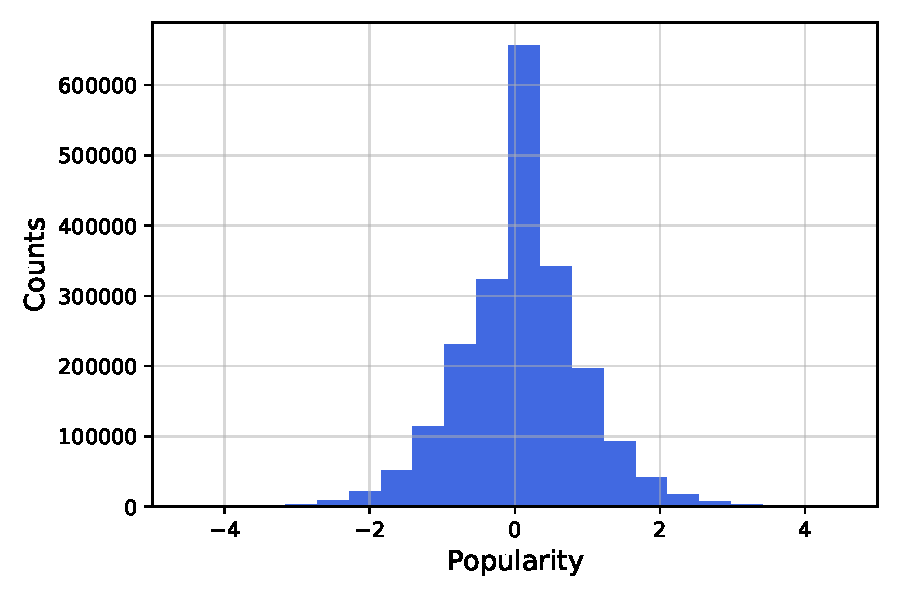
\includegraphics[height=4cm]{Pictures/PopularityDist.pdf}
    \caption{Popularity distribution}
    \label{PopDist}
    \end{subfigure}%
\hfill
    \begin{subfigure}{0.5\tw}
    \centering
    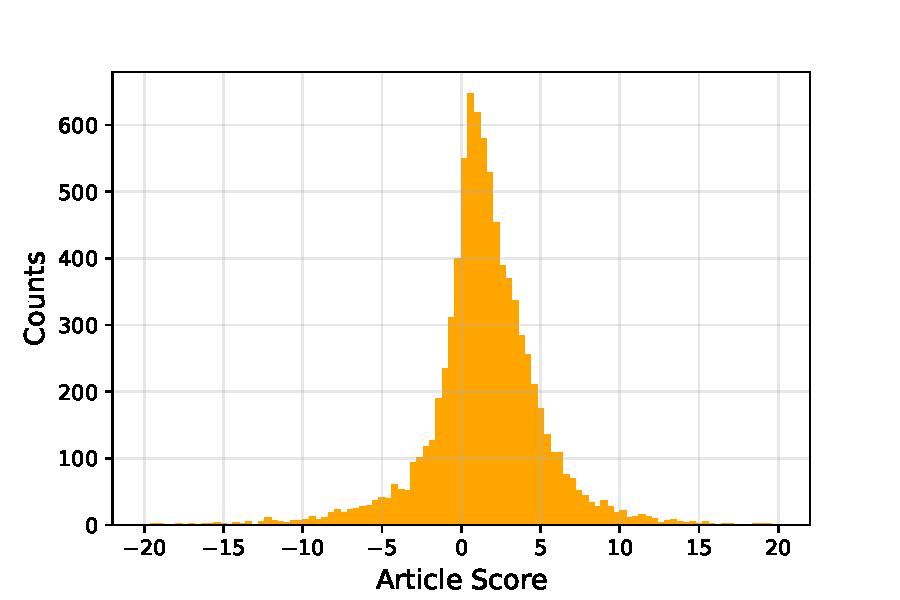
\includegraphics[height=4.5cm]{Pictures/articleScoreDist.pdf}
    \caption{Article score distribution.}
    \label{AScore}
    \end{subfigure}
\caption{Preliminary distributions.}
\end{figure}

The article score distribution shows a similar behaviour; it is reported in Fig. \ref{AScore} even though it will not be included in further analyses. Again, the article Score calculated with Eq. \ref{ASeq} shows a quite symmetrical distribution, meaning that the estimator is consistent and the articles are distributed equally among the polarity spectrum.

\subsection{Strategy 1 (linear)}
The first strategy to estimate controversy in news articles (Eq. \ref{Str1}) was to multiply the number of comments related to each article with the IQR of the popularity distribution for such comments (labelled as \textit{debate}). This calculation lead to an index of controversy peaked near 0. Furthermore, the controversy distribution looks very similar to the comment number distribution (see Fig. \ref{Str1Dist}). This suggests that popularity and controversy are strongly correlated, while debate plays an insignificant role in the compute. 

\begin{figure}[tb]
\centering
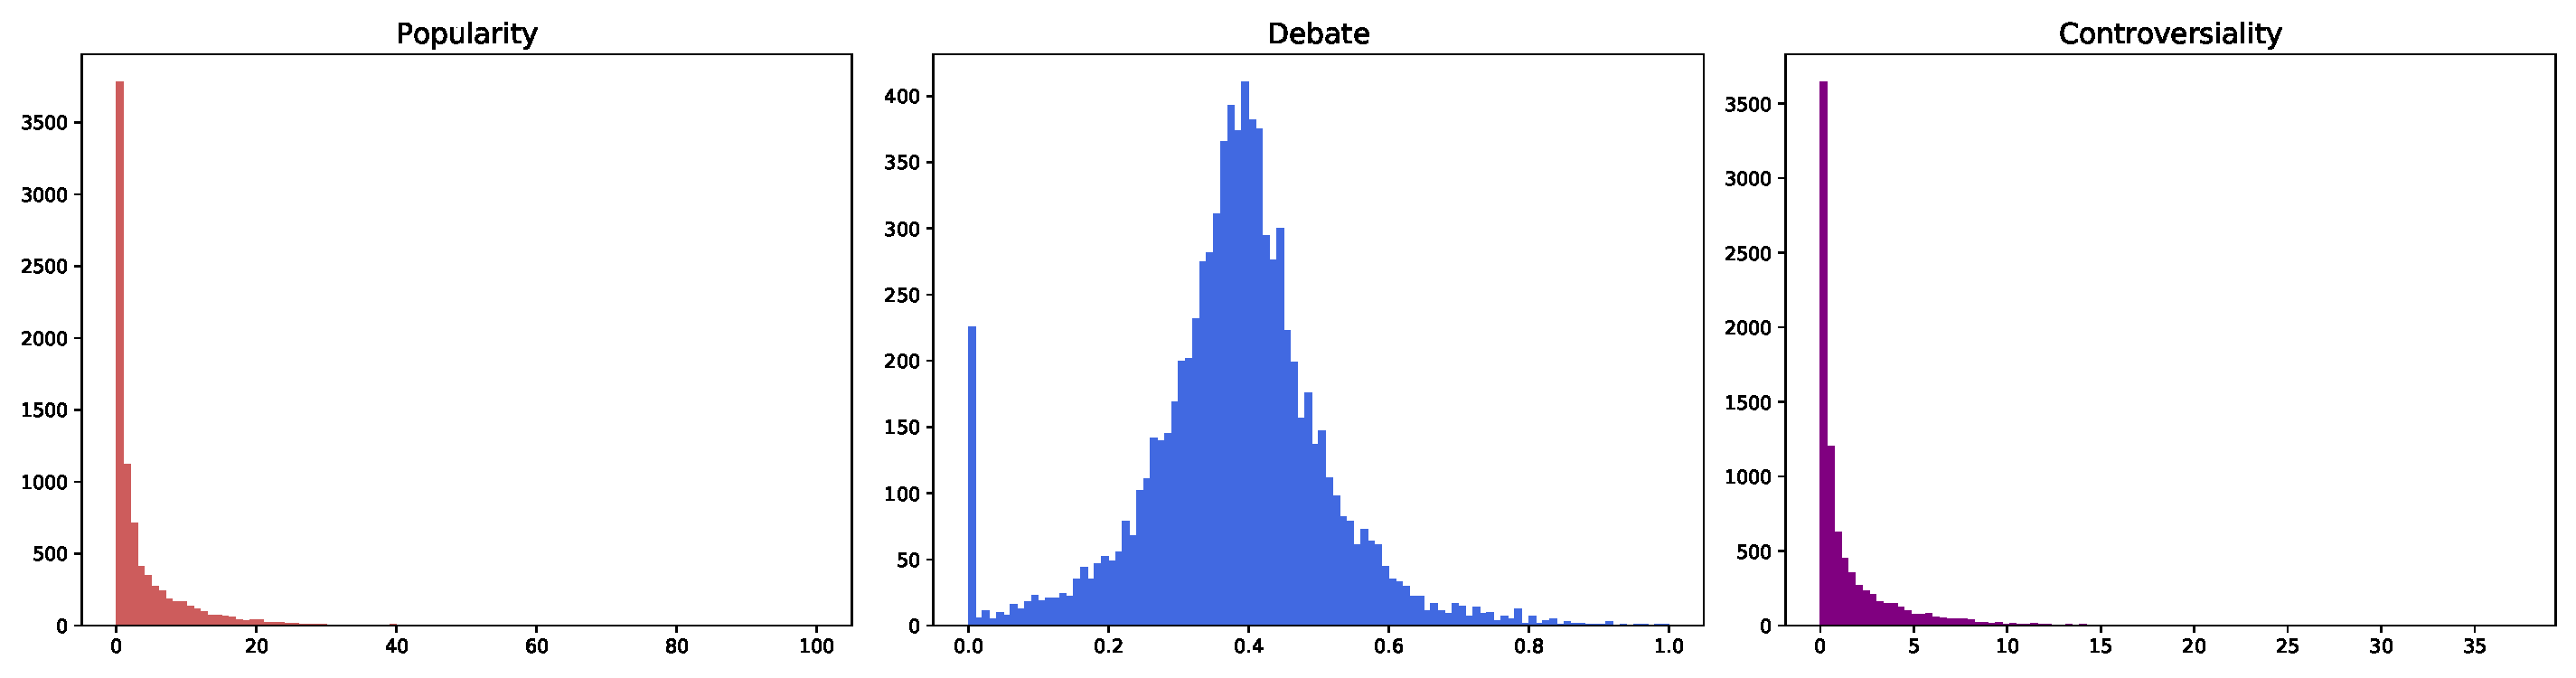
\includegraphics[width=\tw]{Pictures/Strat1Dist.pdf}
\caption{Popularity, Debate and Controversy distributions for Strategy 1}
\label{Str1Dist}
\end{figure}

To corroborate this hypothesis, the correlation scatter plots for the three variables were built, and Fig. \ref{Str1Corr} shows a very strong linear correlation between popularity and controversy. This correlation rows against the thesis of the project, which is trying to differentiate the so-called "hot topics" from the most controversial ones. For this reason, another strategy was implemented to see if some other definition of controversy can detach more efficiently from the concept of popularity.

\begin{figure}[tb]
\centering
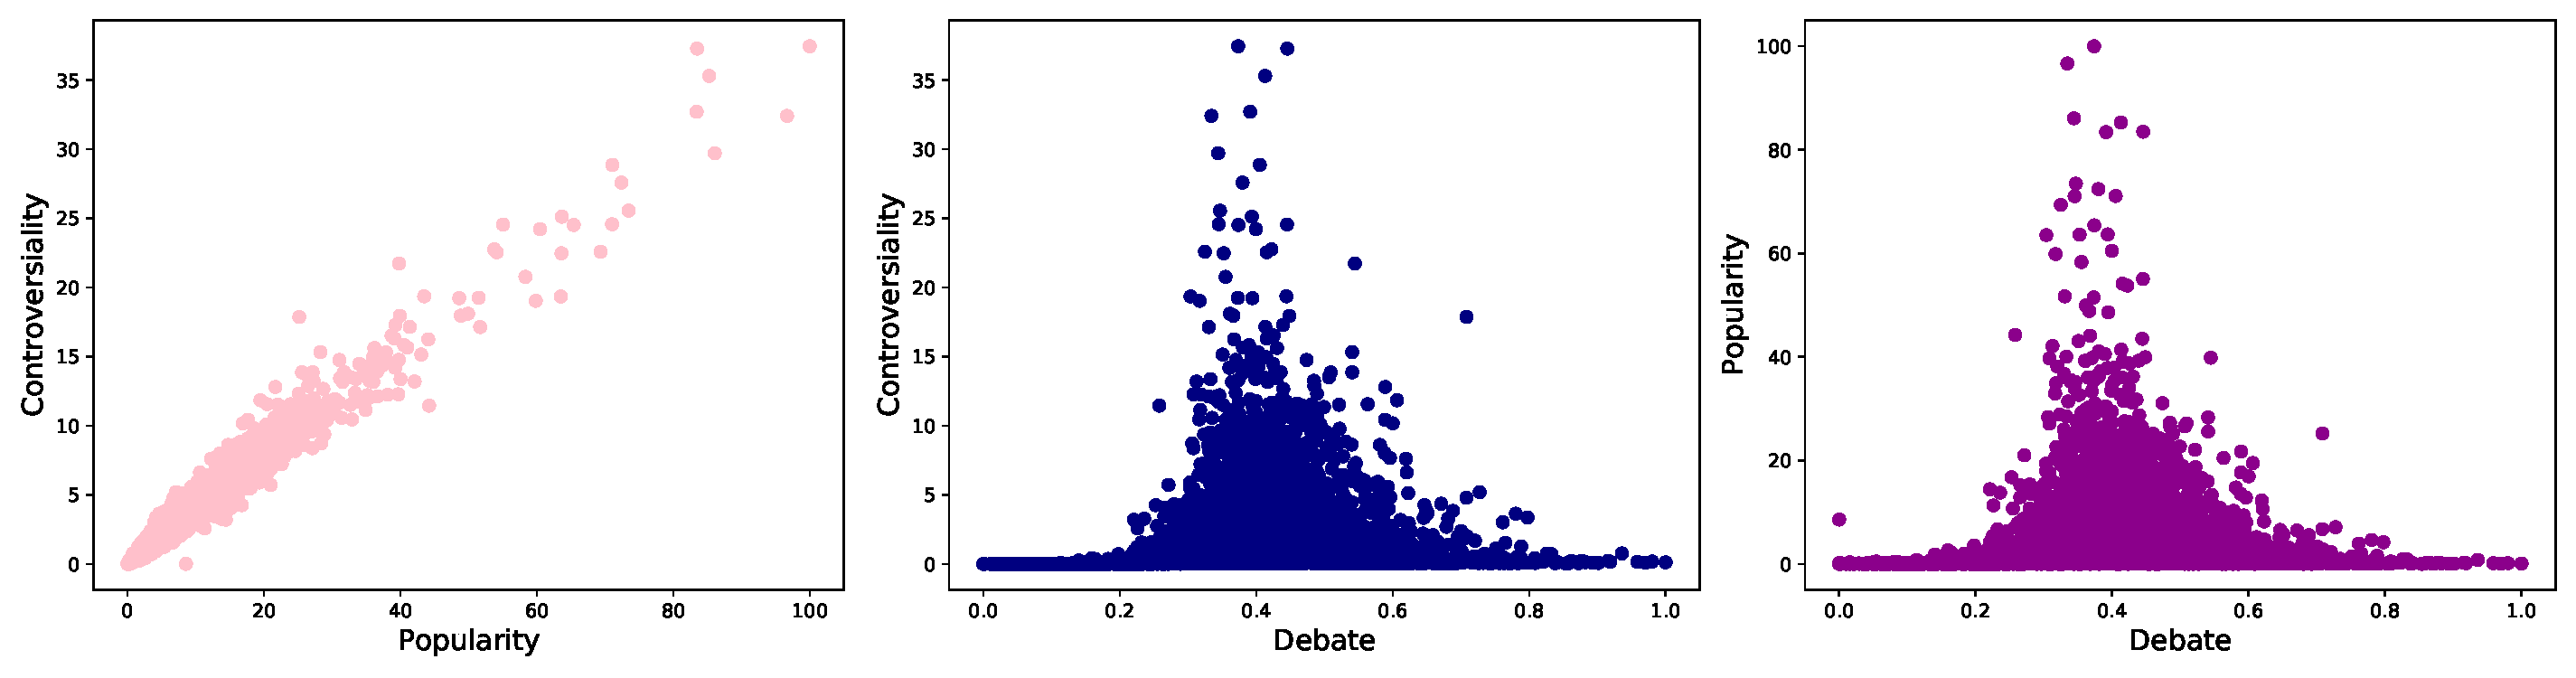
\includegraphics[width=\tw]{Pictures/Strat1Corr.pdf}
\caption{Correlation plots for Strategy 1.}
\label{Str1Corr}
\end{figure}

To go deeper into the analysis, the controversy scores for each articles were averaged among articles of the same section. This grouping was made to see if any article section is more controversial than others. Unfortunately, Strategy 1 did not prove to be useful in this case, as the most controversial topics are also the most popular one. Figure \ref{RG1} shows how, for each section, the controversy and the popularity score look very similar to each other (after proper normalisation).

\begin{figure}
\centering
\includegraphics
\end{figure}
\begin{thebibliography}{15}

\vspace{1cm}

\bibitem{News_1}
T. B. Magadza and Addlight Mukwazvure and K. P. Supreethi,
  \textit{Exploring Sentiment Classification Techniques in News Articles}, IJITKM Vol. 8, no. 1, pp. 55-58, 2014
\bibitem{News_2}
P. Raina, \textit{Sentiment Analysis of News Articles Using Sentic Computing}, 2013 IEEE 13th Int. Conf. Data Min. Work., pp. 959-962, 2013

\bibitem{Guardian}
A. Mukwazvure and K. P. Supreethi \textit{A hybrid approach to sentiment analysis of news comments}, 4th International Conference on Reliability, 2015

\bibitem{Chinese}
W. Fan and S. Sun, \textit{Sentiment Classification of Online Comments on Chinese News}, International Conference on Computer Applications and System Modeling, 2010

\bibitem{Dataset}
A. Kesarwani, \textit{New York Times Comments Dataset}, \href{https://www.kaggle.com/aashita/nyt-comments}{Kaggle link}

\bibitem{Aggarwal}
C. Aggarwal, \textit{Machine Learning for Text}, Springer 2018

\bibitem{NLTK}
S. Bird, E. Klein and E. Loper, \textit{Natural language processing with Python: analyzing text with the natural language toolkit}, O'Reilly Media Inc., 2009

\bibitem{AFINN}
F. A. Nielsen, \textit{AFINN}, Informatics Math. Model Tech. Univ. Denamrk, 2011


\end{thebibliography}

\end{document}
